%!TEX TS-program = xelatex

\documentclass[t]{beamer}

\usetheme{Hannover}
\usecolortheme{rose}

\usepackage{fontspec,xltxtra,xunicode}      %% подготавливает загрузку шрифтов Open Type, True Type и др.
%\defaultfontfeatures{Ligatures={TeX},Renderer=Basic}  %% свойства шрифтов по умолчанию
\setmainfont[Ligatures={TeX,Historic},
SmallCapsFont={Brill},
SmallCapsFeatures={Letters=SmallCaps}]{Brill} %% задаёт основной шрифт документа
\setsansfont{Brill}                    %% задаёт шрифт без засечек
\setmonofont[Ligatures=NoCommon]{DejaVu Sans}
\newfontfamily\SYM{Brill}
\usepackage{indentfirst}
%%% Дополнительная работа с математикой
\usepackage{amsmath,amsfonts,amssymb,amsthm,mathtools} % AMS
\usepackage{icomma} % "Умная" запятая: $0,2$ --- число, $0, 2$ --- перечисление

%%% Работа с картинками
\usepackage{wrapfig} % Обтекание рисунков текстом
\usepackage{rotating}
\usepackage{fixltx2e}
\usepackage{hhline}
\usepackage{lscape}

%%% Работа с таблицами
\usepackage{array,tabularx,tabulary,booktabs} % Дополнительная работа с таблицами
\usepackage{longtable}  % Длинные таблицы
\usepackage{multirow} % Слияние строк в таблице

\usepackage{multicol} % Несколько колонок
%%% Страница
%\usepackage{fancyhdr} % Колонтитулы
% 	\pagestyle{fancy}
 	%\renewcommand{\headrulewidth}{0pt}  % Толщина линейки, отчеркивающей верхний колонтитул
% 	\lfoot{Нижний левый}
% 	\rfoot{Нижний правый}
% 	\rhead{Верхний правый}
% 	\chead{Верхний в центре}
% 	\lhead{Верхний левый}
%	\cfoot{Нижний в центре} % По умолчанию здесь номер страницы

\usepackage{setspace} % Интерлиньяж
%\onehalfspacing % Интерлиньяж 1.5
%\doublespacing % Интерлиньяж 2
\singlespacing % Интерлиньяж 1

\usepackage{subfig} % подкартинки
\usepackage{lastpage} % Узнать, сколько всего страниц в документе.
\usepackage{soul} % Модификаторы начертания
\usepackage{bbding}
\usepackage{tikz} % Работа с графикой
\usepackage{pgfplots}
\usepackage{pgfplotstable}
\usepackage{verbatim}

\usepackage{attachfile2}
\usepackage{alltt}

%%% Лингвистические пакеты
%\usepackage{savetrees} % пакет, который экономит место
\usepackage{forest} % для рисования деревьев
\usepackage{vowel} % для рисования трапеций гласных
\usepackage{natbib}
\bibpunct[: ]{[}{]}{;}{a}{}{,}
\usepackage[nogroupskip,nopostdot, nonumberlist]{glossaries}
%\usepackage{glossary-mcols} 
%\setglossarystyle{mcolindex}
\usepackage{philex} % пакет для примеров
\newcommand{\mytem}{\item[$\circ$]}
\addto\captionsrussian{
\renewcommand{\refname}{}}

\newcommand{\apostrophe}{\XeTeXglyph\XeTeXcharglyph"0027\relax}
\usetikzlibrary{patterns}

\usepackage{ulem}

\usepackage{hyperref}\setbeamercolor{alerted text}{fg=blue}
\setbeamersize{text margin left=4mm,text margin right=1mm} 
\setbeamertemplate{frametitle}[default][center]
\setbeamertemplate{navigation symbols}{
	\usebeamerfont{footline}%
    \usebeamercolor[fg]{footline}%
    \hspace{1em}%
    {{\small презентация доступна: \href{}{\textbf{}}}
    \hspace{4cm}
    \insertframenumber/\inserttotalframenumber\vspace{0.5mm}}}
\title[]{Vowels}
\author[]{G. Moroz}
\date{10 February, 2018}
\begin{document}
\frame{\titlepage}

\begin{frame}{Previously}
\begin{itemize}
\item Sound waves have
\begin{itemize}
\item A --- amplitude
\item f --- fundamental frequency
\item φ --- phase
\item t --- time
\end{itemize}
\item Speech sounds are complex waves
\item Fourier transform --- allows to extract components of the complex wave
\end{itemize}
\end{frame}

\section{Source-Filter Model}
\begin{frame}{Source-Filter Model}
\begin{itemize}
\item Larynx produce some sound
\item Vocal tract filter some frequencies
\end{itemize}
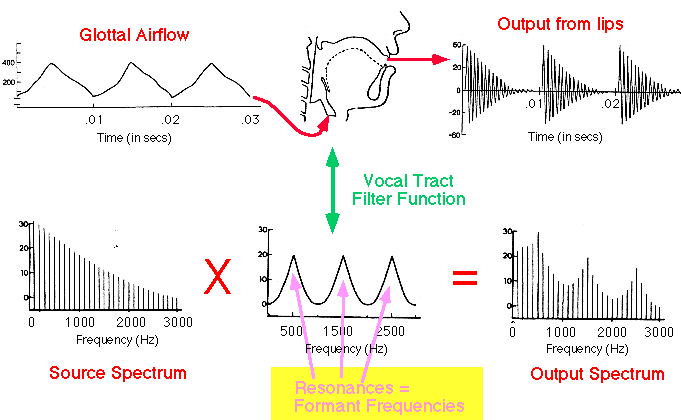
\includegraphics[width=0.95\linewidth]{01-source-filter.png}
\end{frame}

\section{Wave length}

\section{Source-Filter Model}
\begin{frame}{Source-Filter Model of Speech Production}
The output energy (at the mouth) for a given frequency is equal to the amplitude the source harmonic, multiplied by the magnitude of the filter function for that the frequency.
\end{frame}

\begin{frame}{???}
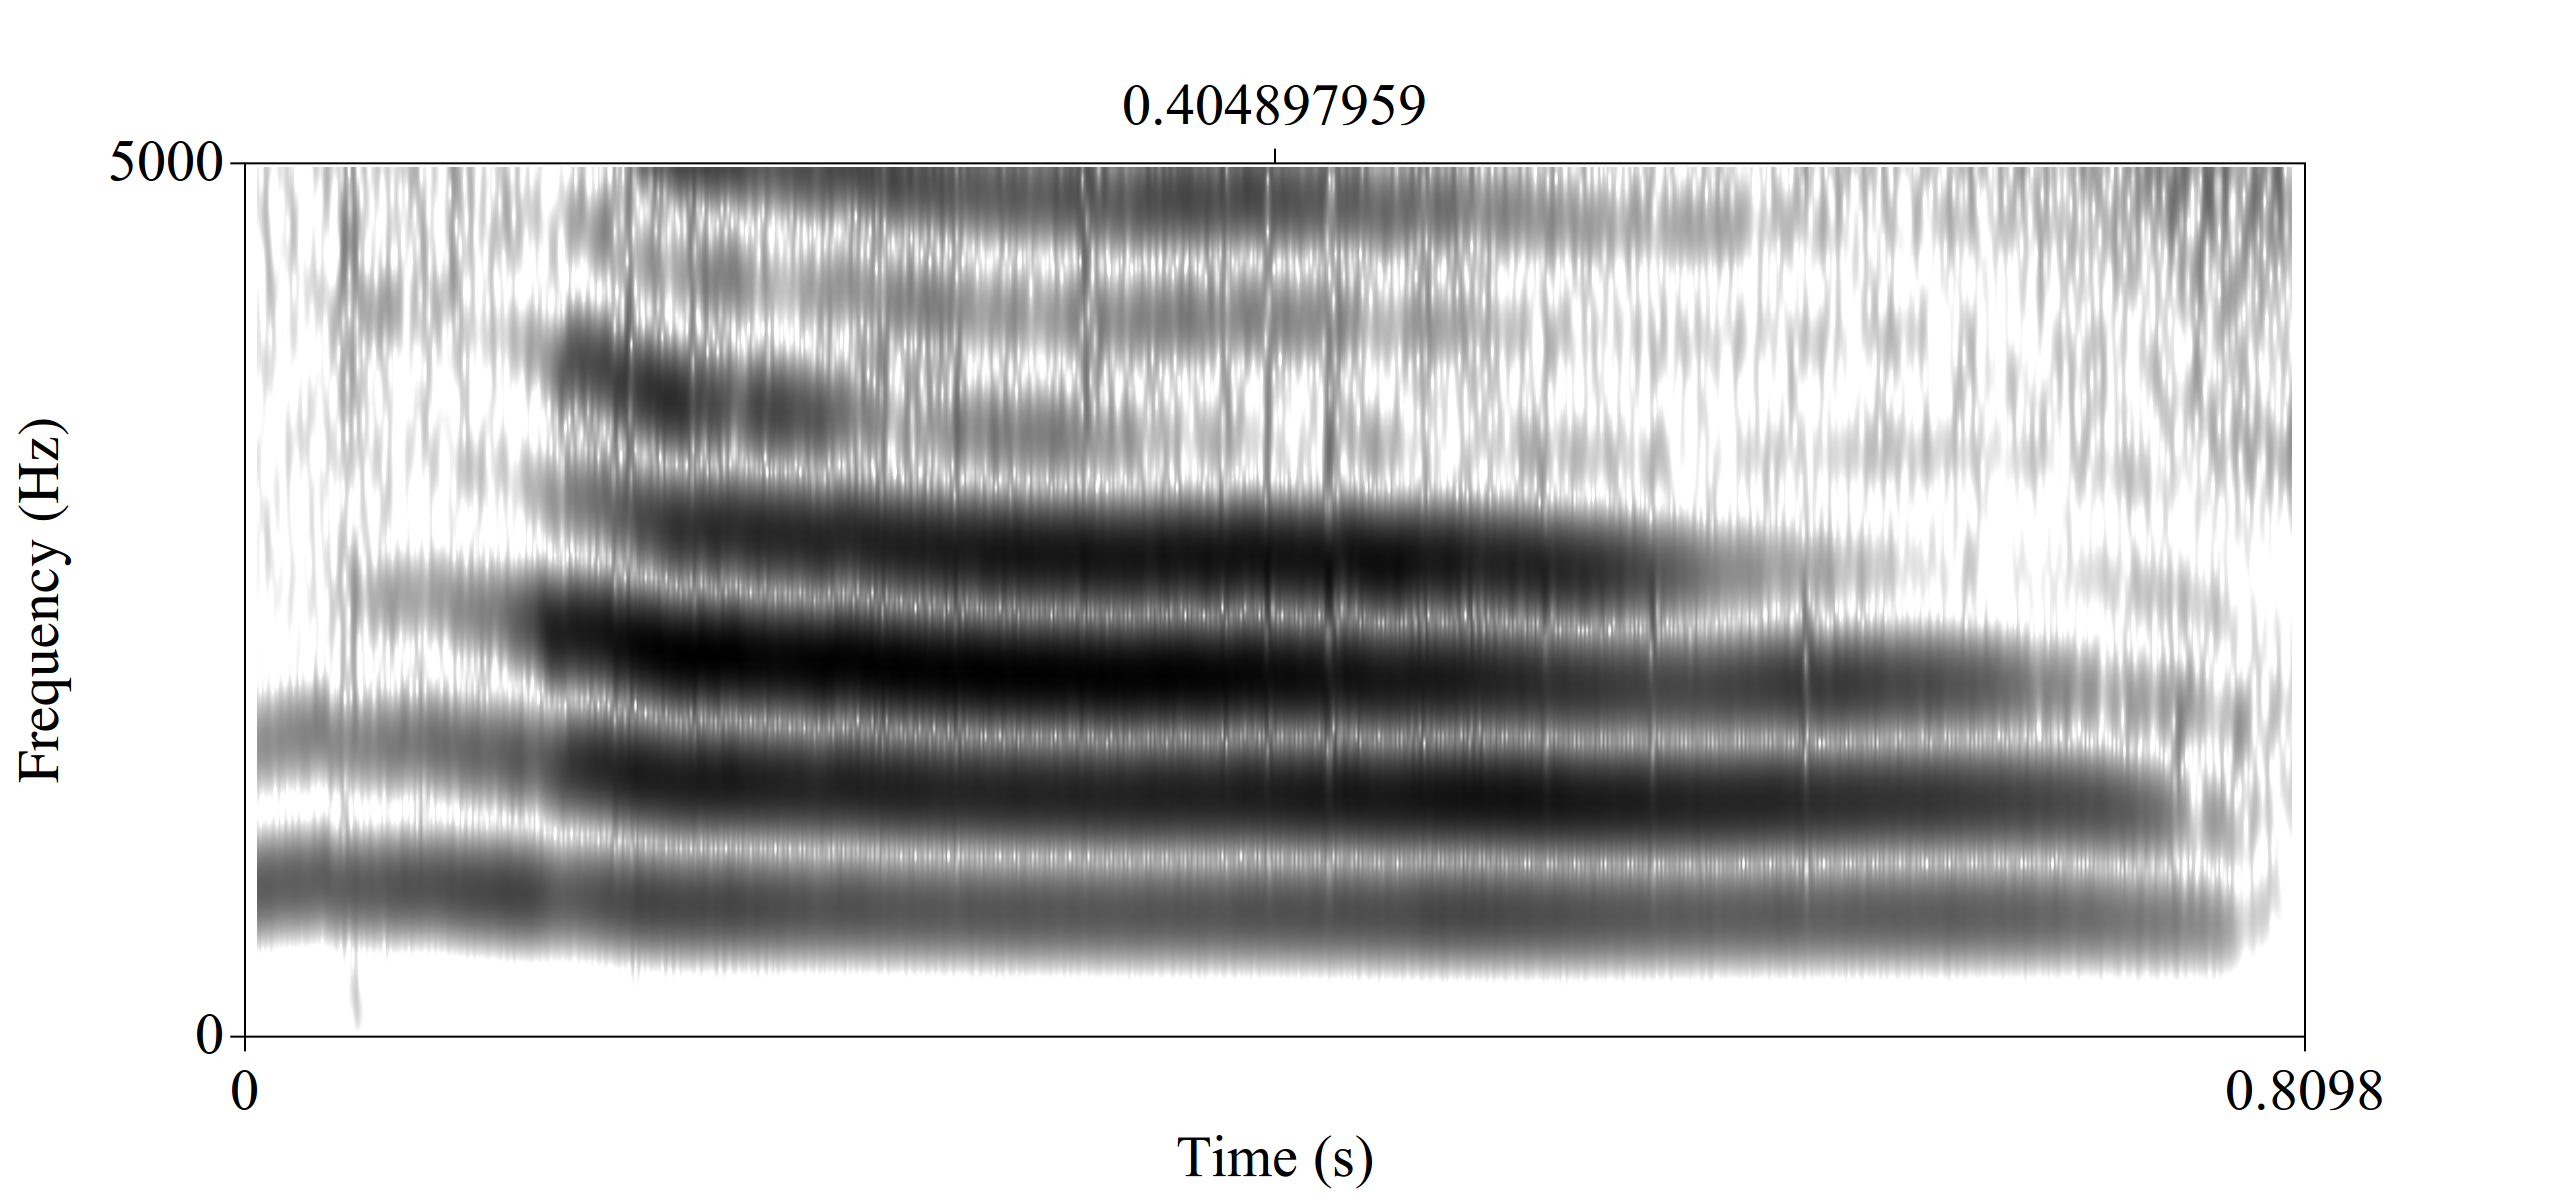
\includegraphics[width=\linewidth]{02-cat-meow.png}
\end{frame}

\begin{frame}{Cat meow}
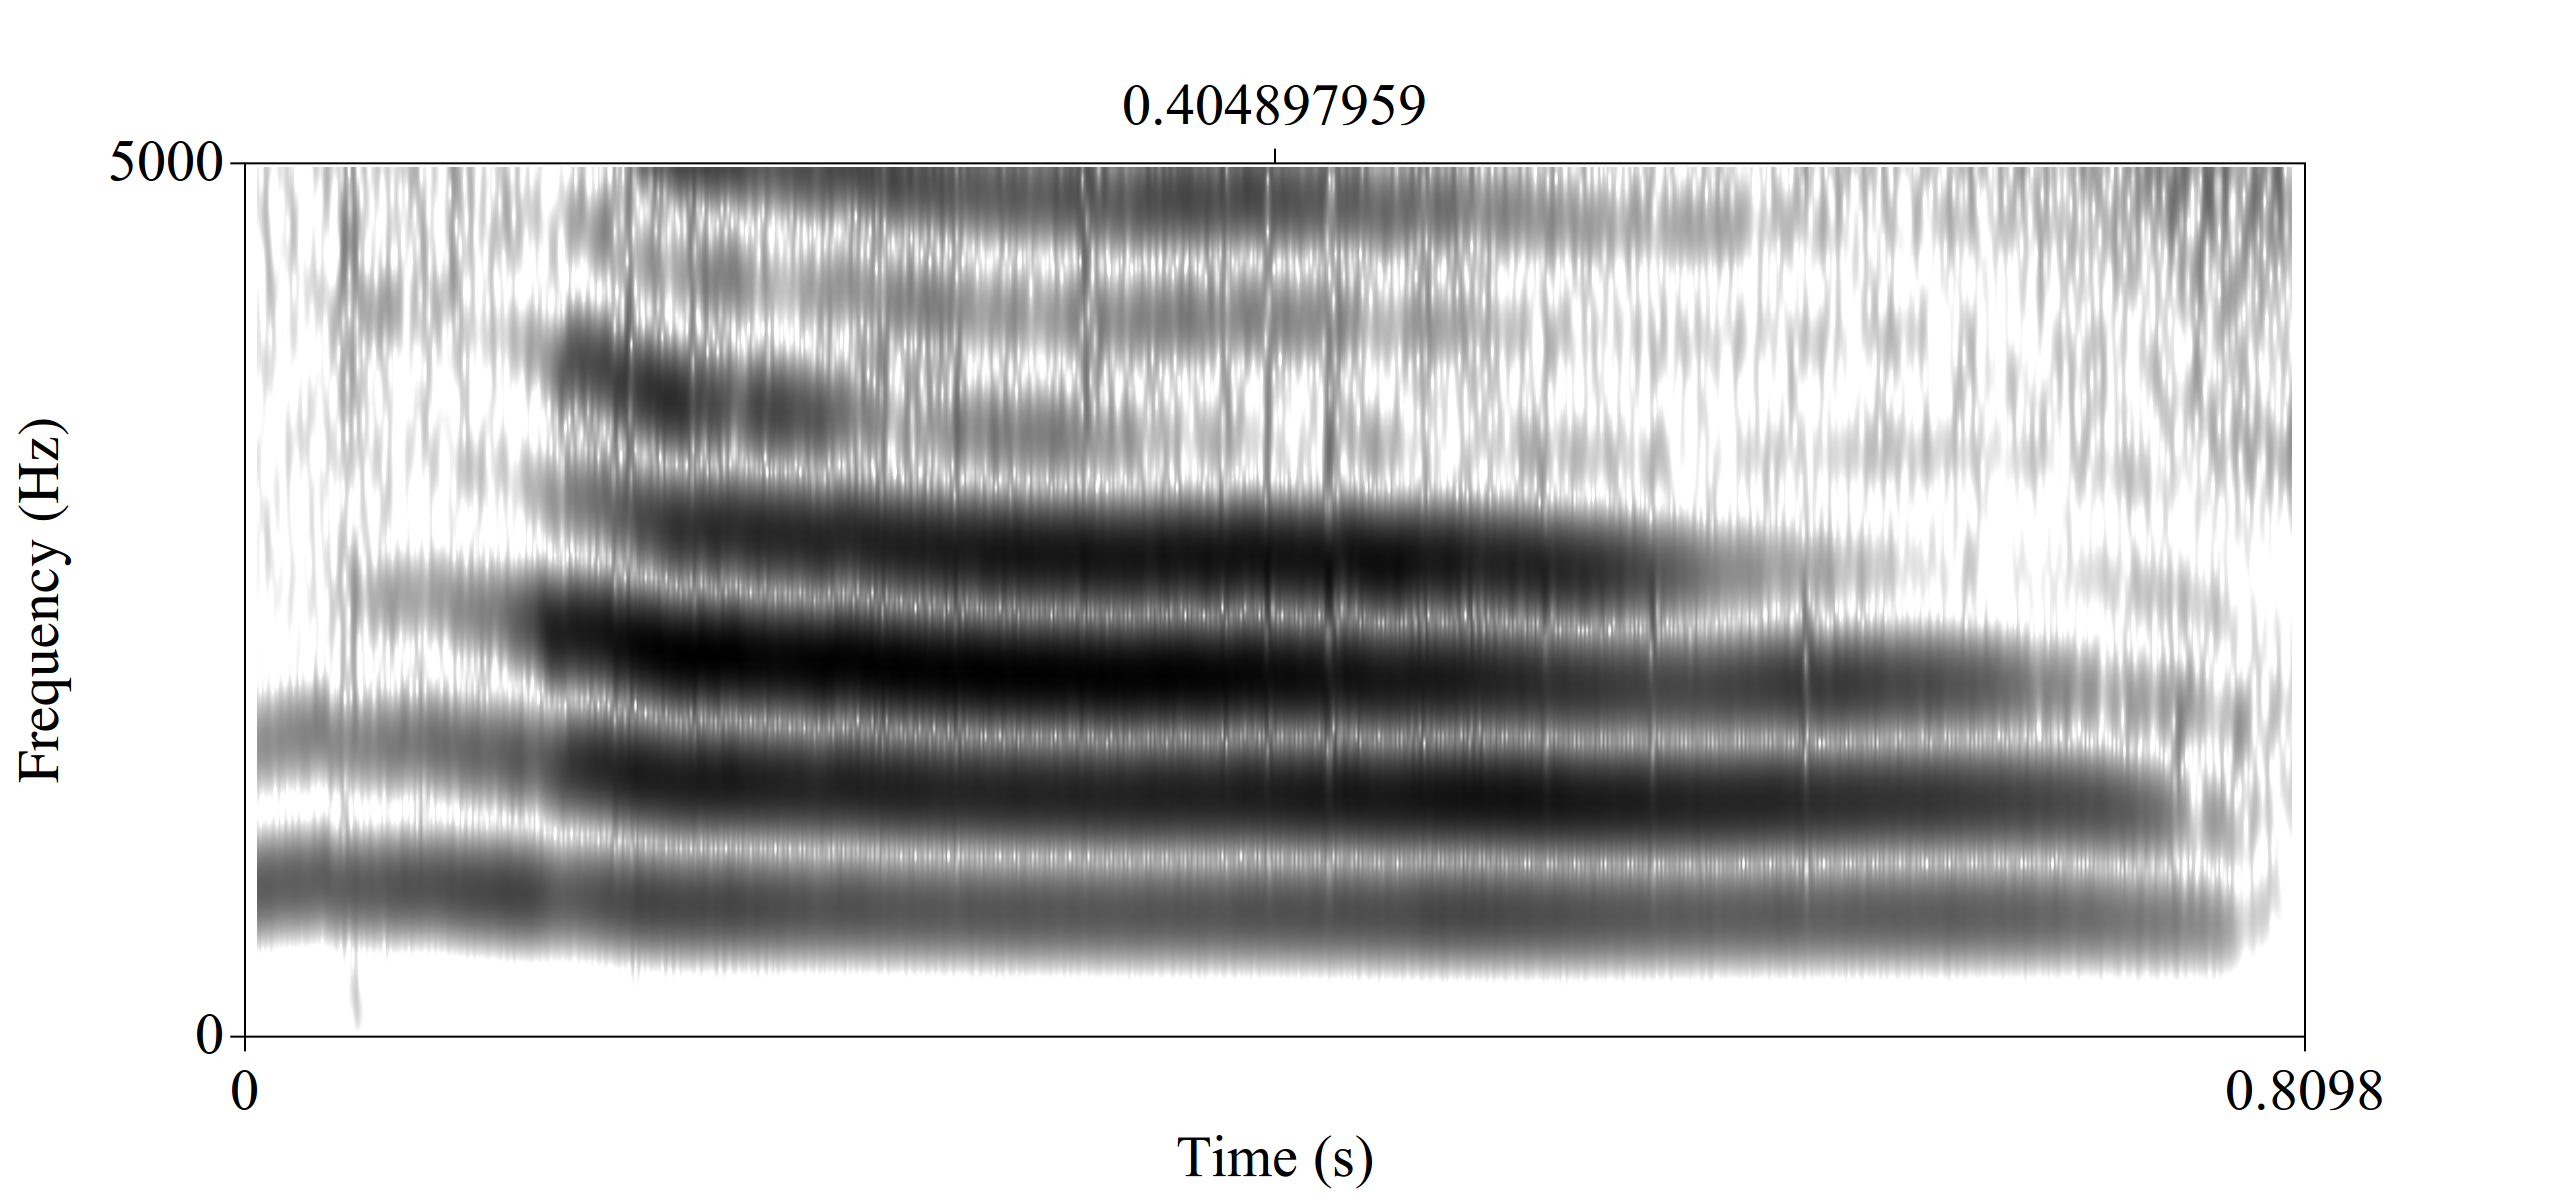
\includegraphics[width=\linewidth]{02-cat-meow.png}
\end{frame}

\begin{frame}{Vowel chart}
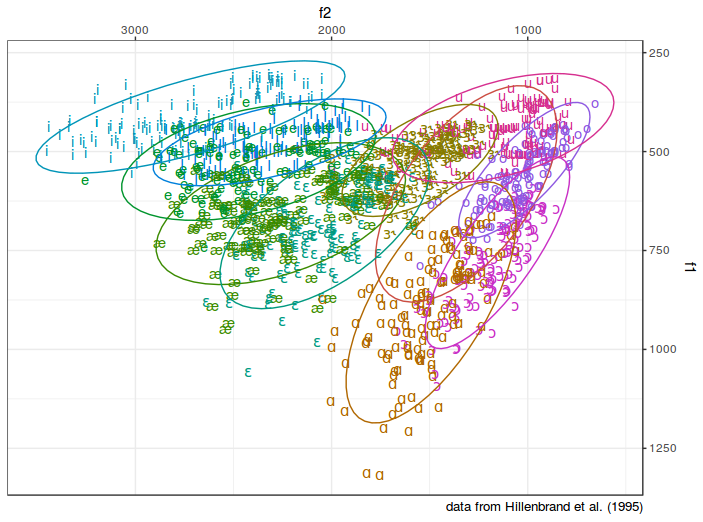
\includegraphics[width=\linewidth]{03-vowel-chart.png}
\end{frame}

\begin{frame}{Vowel editor}
Praat objects > New > Sound > Create sound from VowelEditor...
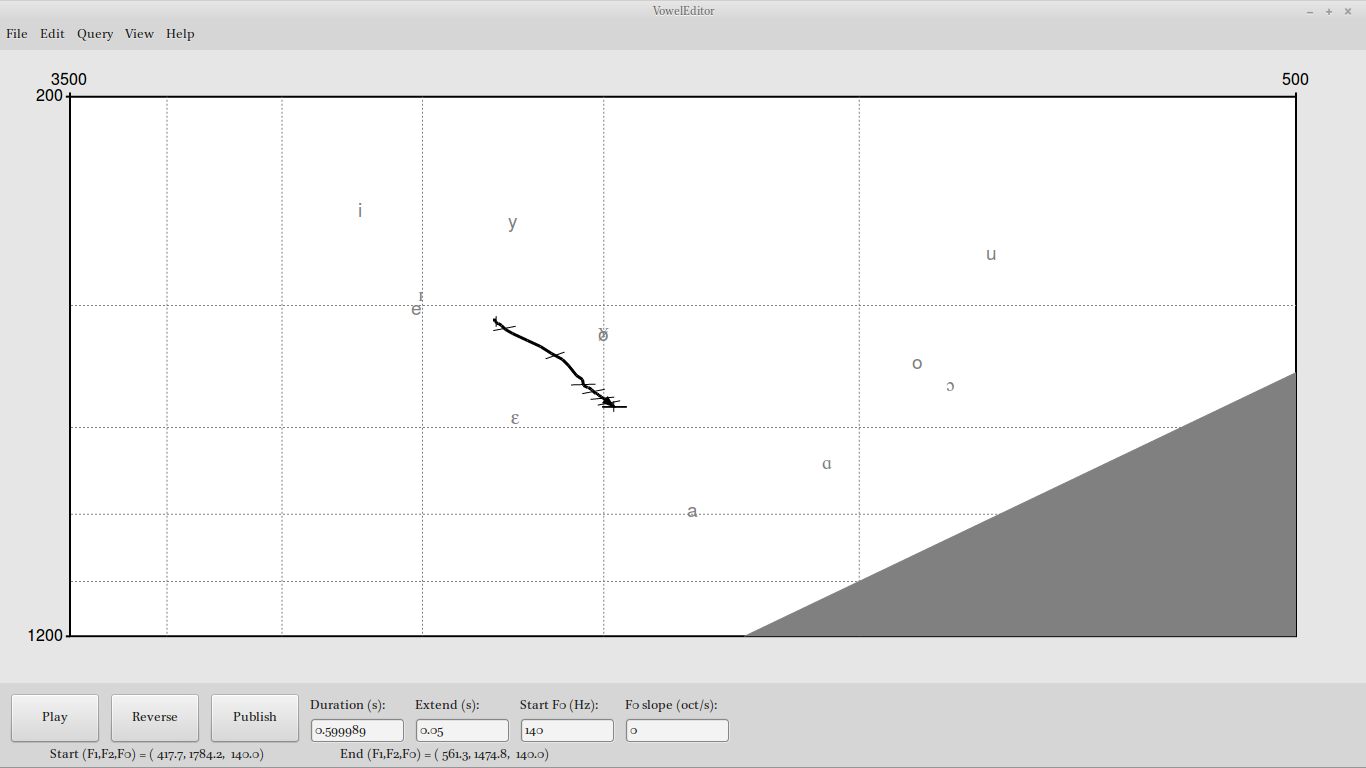
\includegraphics[width=\linewidth]{04-vowel-editor.png}
\end{frame}


\section{Vowel analysis}
\begin{frame}{How to analyse vowels?}
\begin{itemize}
\item record sounds
\item annotate sounds
\item make an exploratory analysis
\item extract duration and formant information from your data
\item create the plot
\end{itemize}
\end{frame}

\begin{frame}{How to analyse vowels?}
\begin{itemize}
\item[\checkmark] record sounds
\item[\checkmark] annotate sounds
\item make an exploratory analysis
\item extract duration and formant information from your data
\item create the plot
\end{itemize}
\end{frame}

\subsection{exploratory analysis}
\begin{frame}{Formants in Praat}
Praat Analyser > Formant > Show Formants\\
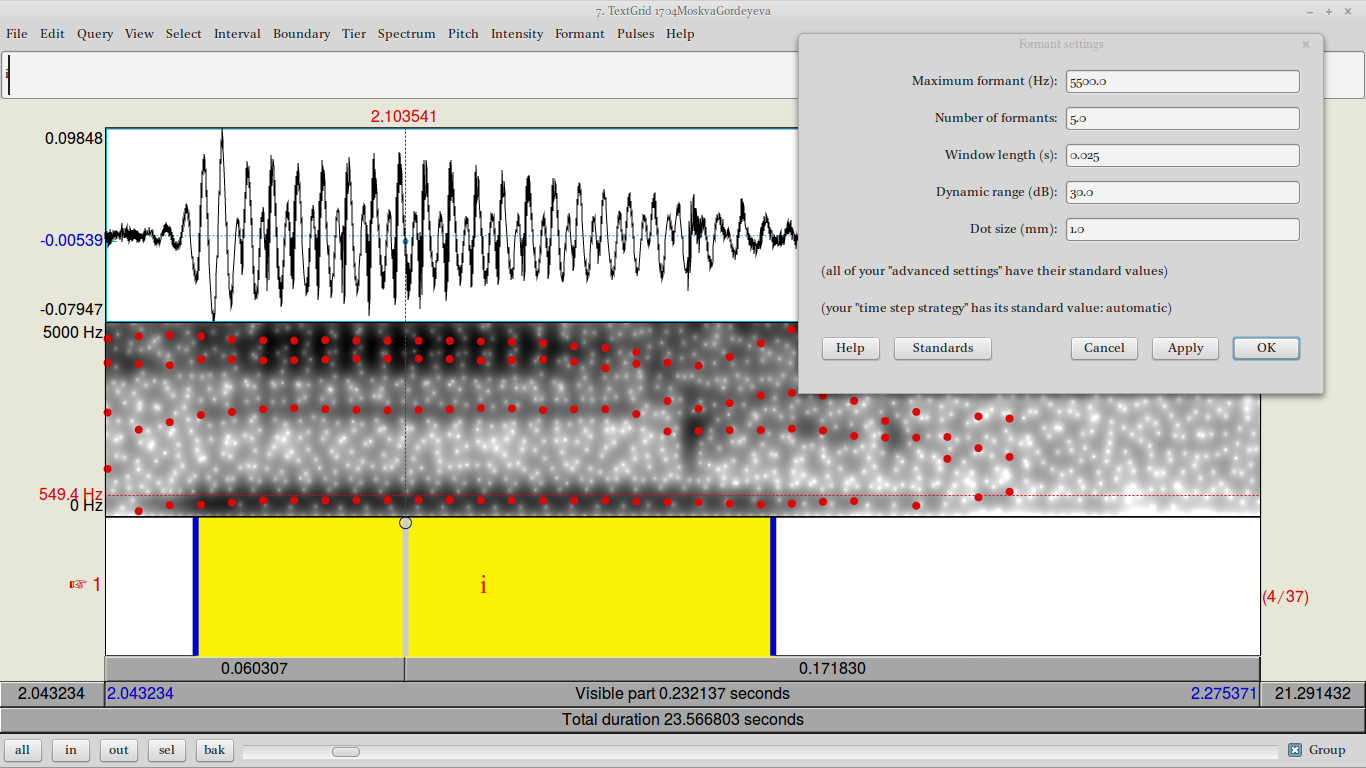
\includegraphics[width=\linewidth]{05-formnats.png}\\
F1 \hfill select the nearest first formant value or mean value for selection\\
F2 \hfill select the nearest second formant value or mean value for selection\\
F3 \hfill select the nearest third formant value or mean value for selection\\
\end{frame}

\begin{frame}{Formants in Praat}
Praat Analyser > Formant > Formant Settings...\\
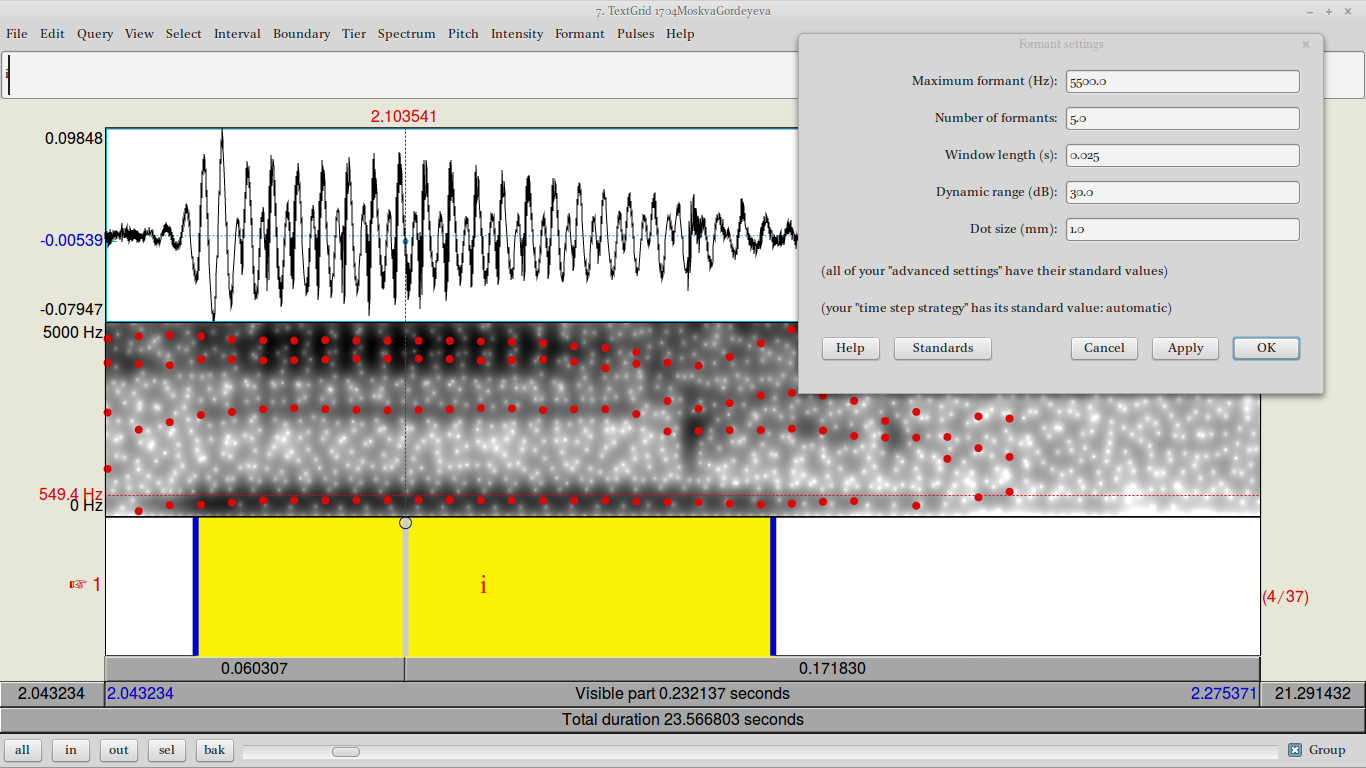
\includegraphics[width=\linewidth]{05-formnats.png}\\
During analysis you should set Maximum Formant value  so as to distinguish [i], [a] and [u].
\end{frame}

\begin{frame}{How to analyse vowels?}
\begin{itemize}
\item[\checkmark] record sounds
\item[\checkmark] annotate sounds
\item[\checkmark] make an exploratory analysis
\item extract duration and formant information from your data
\item create the plot
\end{itemize}
\end{frame}

\subsection{extract data}
\begin{frame}{Change writing preferences to UTF-8!}
Praat Objects > Preferences > Text writing preferences...
\end{frame}

\begin{frame}{Praat scripting}
Praat have its own scripting language. You can read about it:\\
Praat Objects > Help > Scripting tutorial\\
There are  a lot of Praat scripts \href{http://phonetics.linguistics.ucla.edu/facilities/acoustic/praat.html}{here}.
\end{frame}

\begin{frame}{Praat scripting: extracting duration}
\begin{itemize}
\item Open Praat Objects
\item Open some TextGrid
\item Praat Objects > Praat > New Praat script
\item Copy script from \href{https://goo.gl/n7vbDy}{here} to the new window
\item Select TextGrid
\item Praat Script > Run > Run
\item Provide some valid path for the result file
\item Press OK
\end{itemize}
\end{frame}

\begin{frame}{Praat scripting: extracting formant values}
\begin{itemize}
\item Open Praat Objects
\item Praat Objects > Praat > New Praat script
\item Copy script from \href{https://goo.gl/MUBpPw}{here} to the new window
\item Praat Script > Run > Run
\item Provide some path with your sound and TextGrid
\item Provide Maximum Formant value
\item Press OK
\end{itemize}
\end{frame}

\begin{frame}{How to analyse vowels?}
\begin{itemize}
\item[\checkmark] record sounds
\item[\checkmark] annotate sounds
\item[\checkmark] make an exploratory analysis
\item[\checkmark] extract duration and formant information from your data
\item create the plot
\end{itemize}
\end{frame}

\subsection{plotting}
\begin{frame}[fragile]{Plotting formant values with ggplot2}
\scriptsize
\begin{verbatim}
library(ggplot2)
setwd("...") # Put here path with the result.tsv file
df <- read.csv("result.txt", sep = "\t", fileEncoding = "UTF-8")
ggplot(data = df, aes(F2, F1, color = intervalname, label = intervalname))+
  geom_text(show.legend = F)+
  scale_y_reverse(position = "right")+
  scale_x_reverse(position = "top")
\end{verbatim}
\end{frame}

\begin{frame}[fragile]{Plotting formant values with ggplot2}
\begin{center}
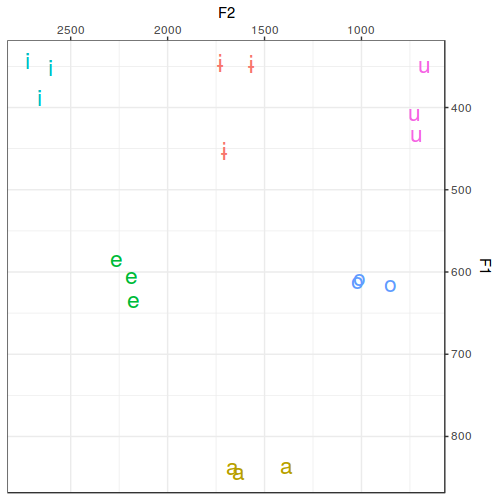
\includegraphics[width=0.7\linewidth]{06-ggplot.png}
\end{center}
\end{frame}

\begin{frame}{How to analyse vowels?}
\begin{itemize}
\item[\checkmark] record sounds
\item[\checkmark] annotate sounds
\item[\checkmark] make an exploratory analysis
\item[\checkmark] extract duration and formant information from your data
\item[\checkmark] create the plot
\end{itemize}
\end{frame}

\section{R packages}
\subsection{vowels}
\begin{frame}{vowels}
\begin{itemize}
\item Version: 1.2-1
\item Date: 2014-11-14
\item Author: Tyler Kendall and Erik R. Thomas, \citep{kendall14}
\end{itemize}
\vfill
\texttt{install.packages("vowels")}
\end{frame}

\subsection{phonTools}
\begin{frame}{phonTools}
\begin{itemize}
\item Version: 0.2-2.1
\item Date: 2015-07-30
\item Author: Santiago Barreda, \citep{barreda15}
\end{itemize}
\vfill
\texttt{install.packages("phonTools")}
\end{frame}

\section{}
\begin{frame}
{\huge Thank you!\bigskip\\
\normalsize Please, don't hesitate to write me\\
agricolamz@gmail.com
\vspace{-130pt}}
\end{frame}
\begin{frame}{Reference}
\footnotesize
\bibliographystyle{chicago}
\bibliography{bibliography}
\end{frame}
\end{document}
